\documentclass[a4j]{jsarticle}
\usepackage{graphicx}
\usepackage{listings}

\title{2024年度プログラミング\textsc{iii} 演習課題}
\author{学籍番号: 35714121 \\ 氏名: 福富隆大}
\date{2024年11月7日}

\begin{document}
\maketitle

\textbf{1 はじめに} \\

本レポートは演習課題第6回の実行結果をまとめたものである。\\

\textbf{2 課題の実行結果} \\

\textmd{(課題6-1)} \\

課題の実行結果を図1に示す。 \\

\begin{figure}[htbp]
  \centering 
  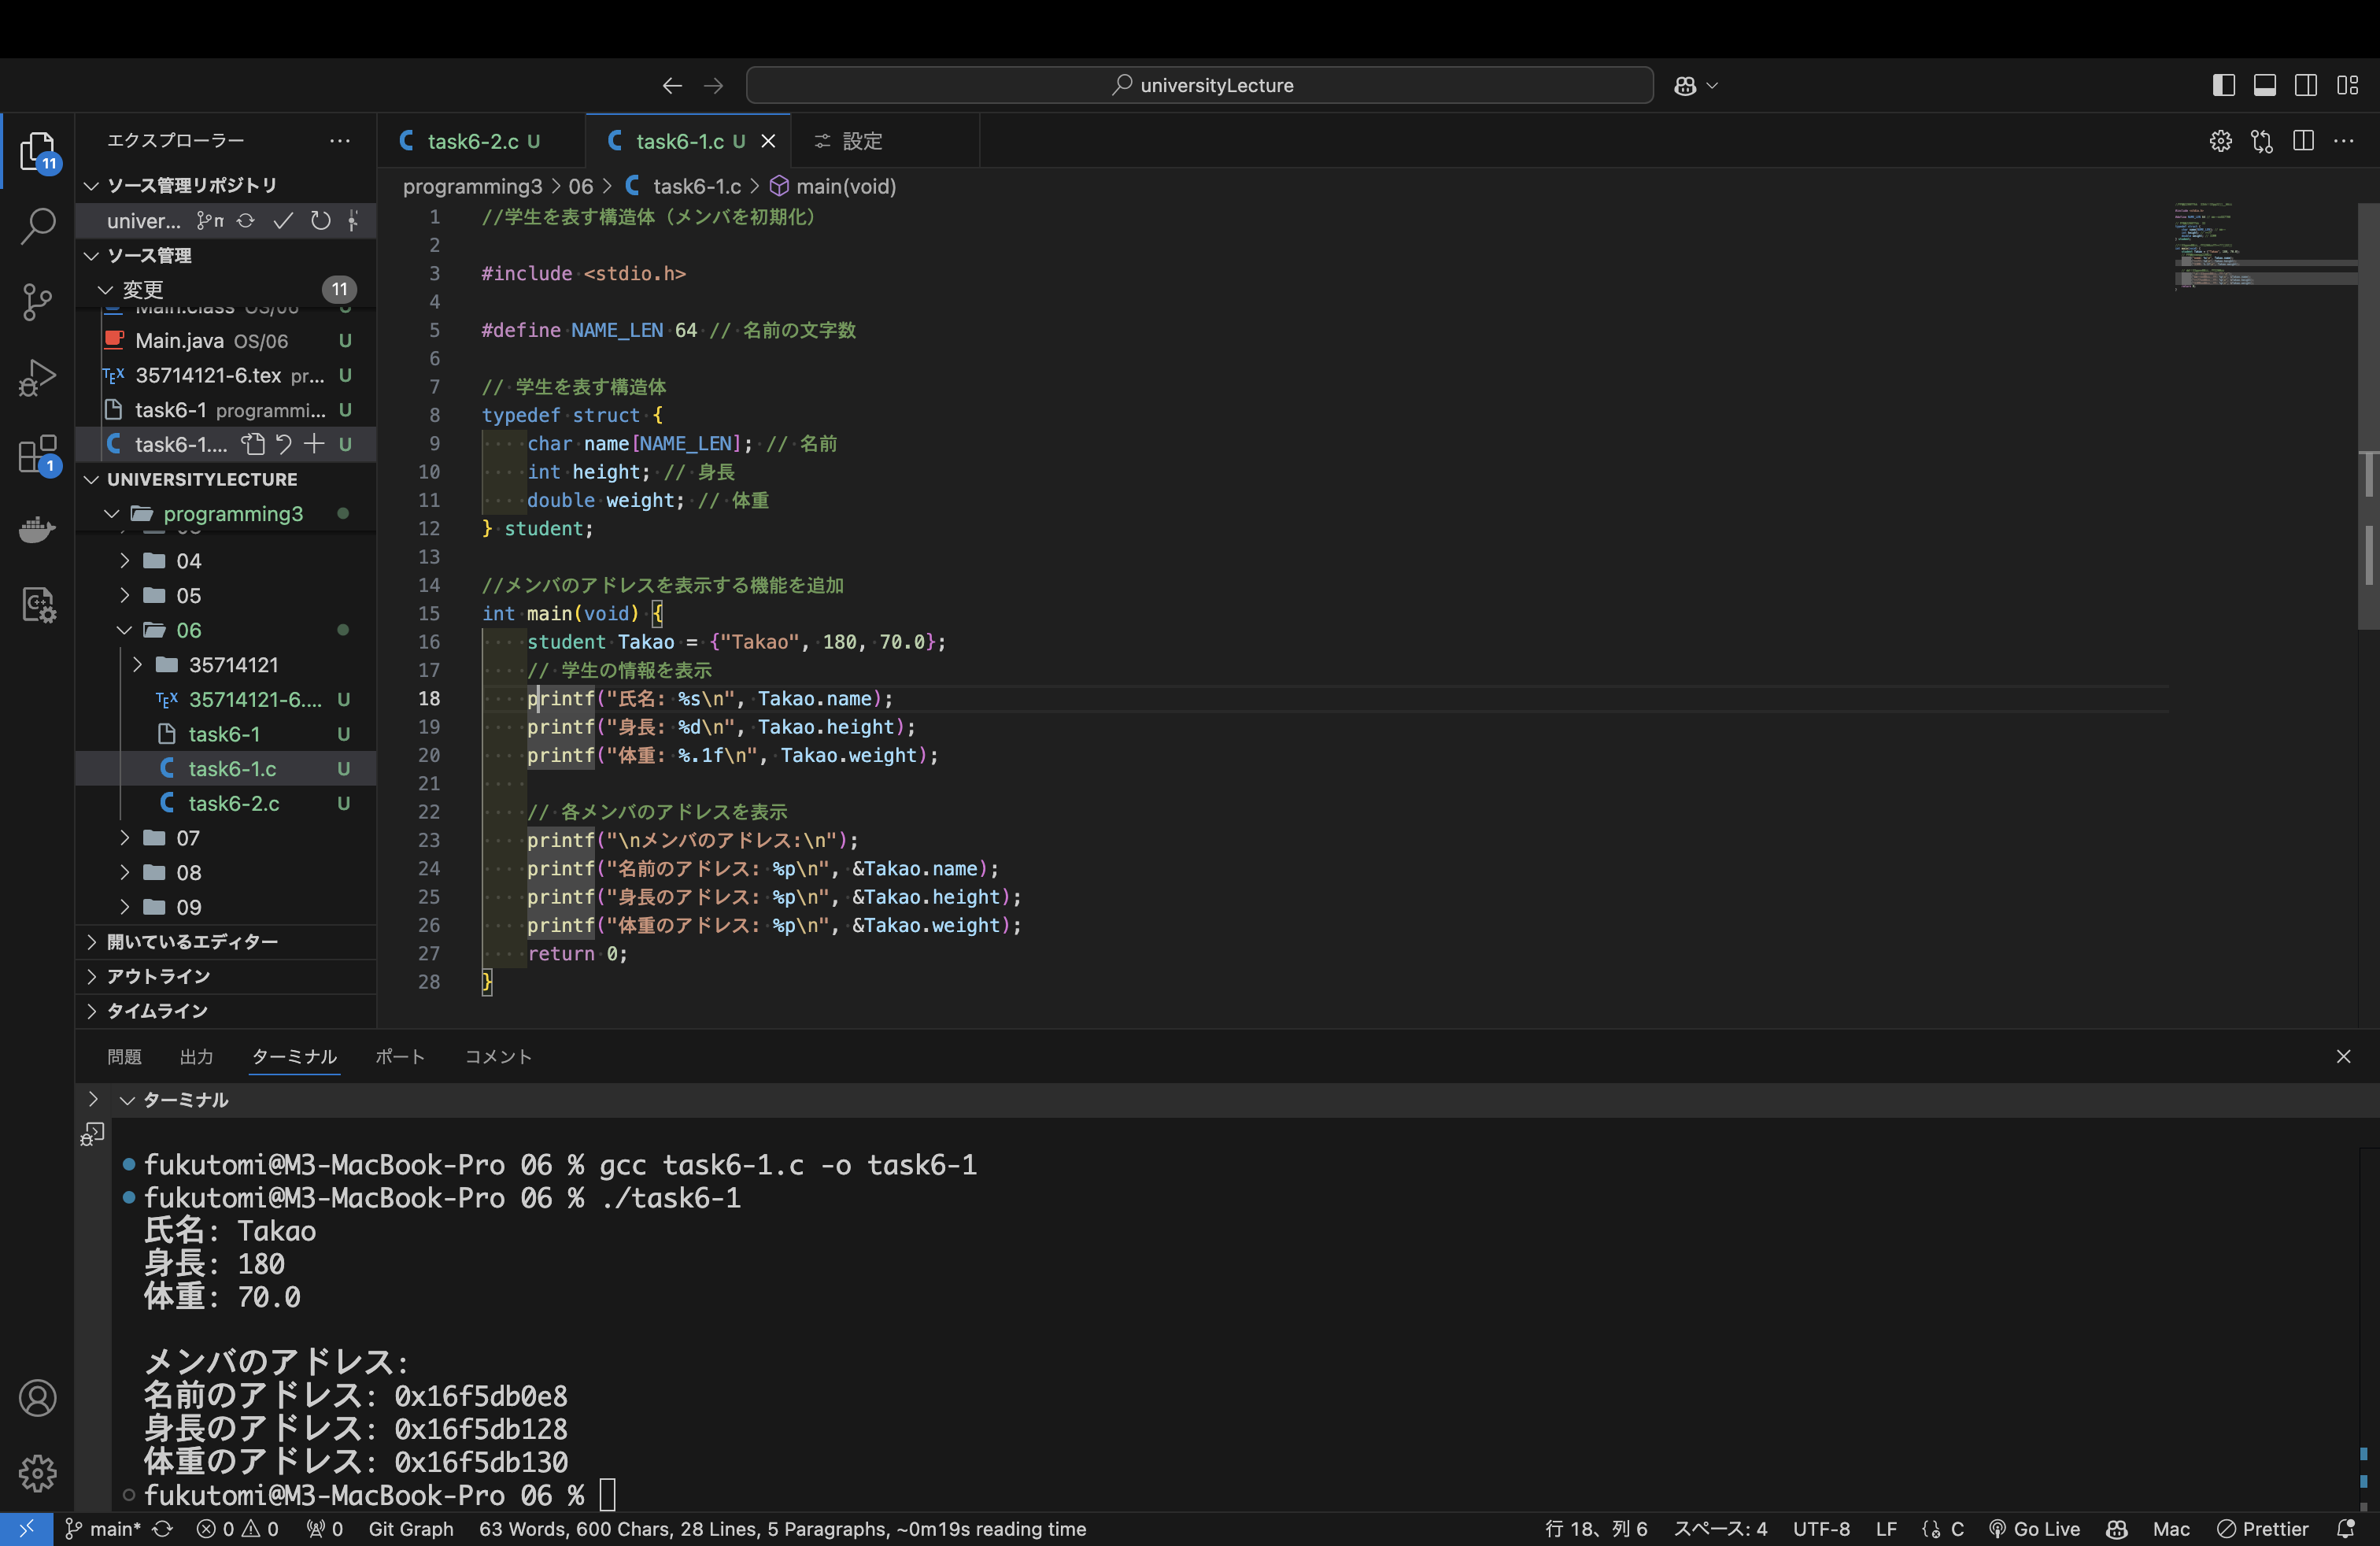
\includegraphics[width=10cm]{task6-1.eps}
  \caption{(ターミナルの部分に実行結果があります)}
  \label{fig:sample1} % ラベル名を変更
\end{figure}

\textmd{コードと結果の説明} \\
メンバのアドレスを表示するには、アドレス演算子\&を使えばいいので、printf("\%p", \&変数名)とした。\\

\textmd{(課題6-2)} \\

課題の実行結果を図2に示す。\\

\begin{figure}[htbp]
  \centering
  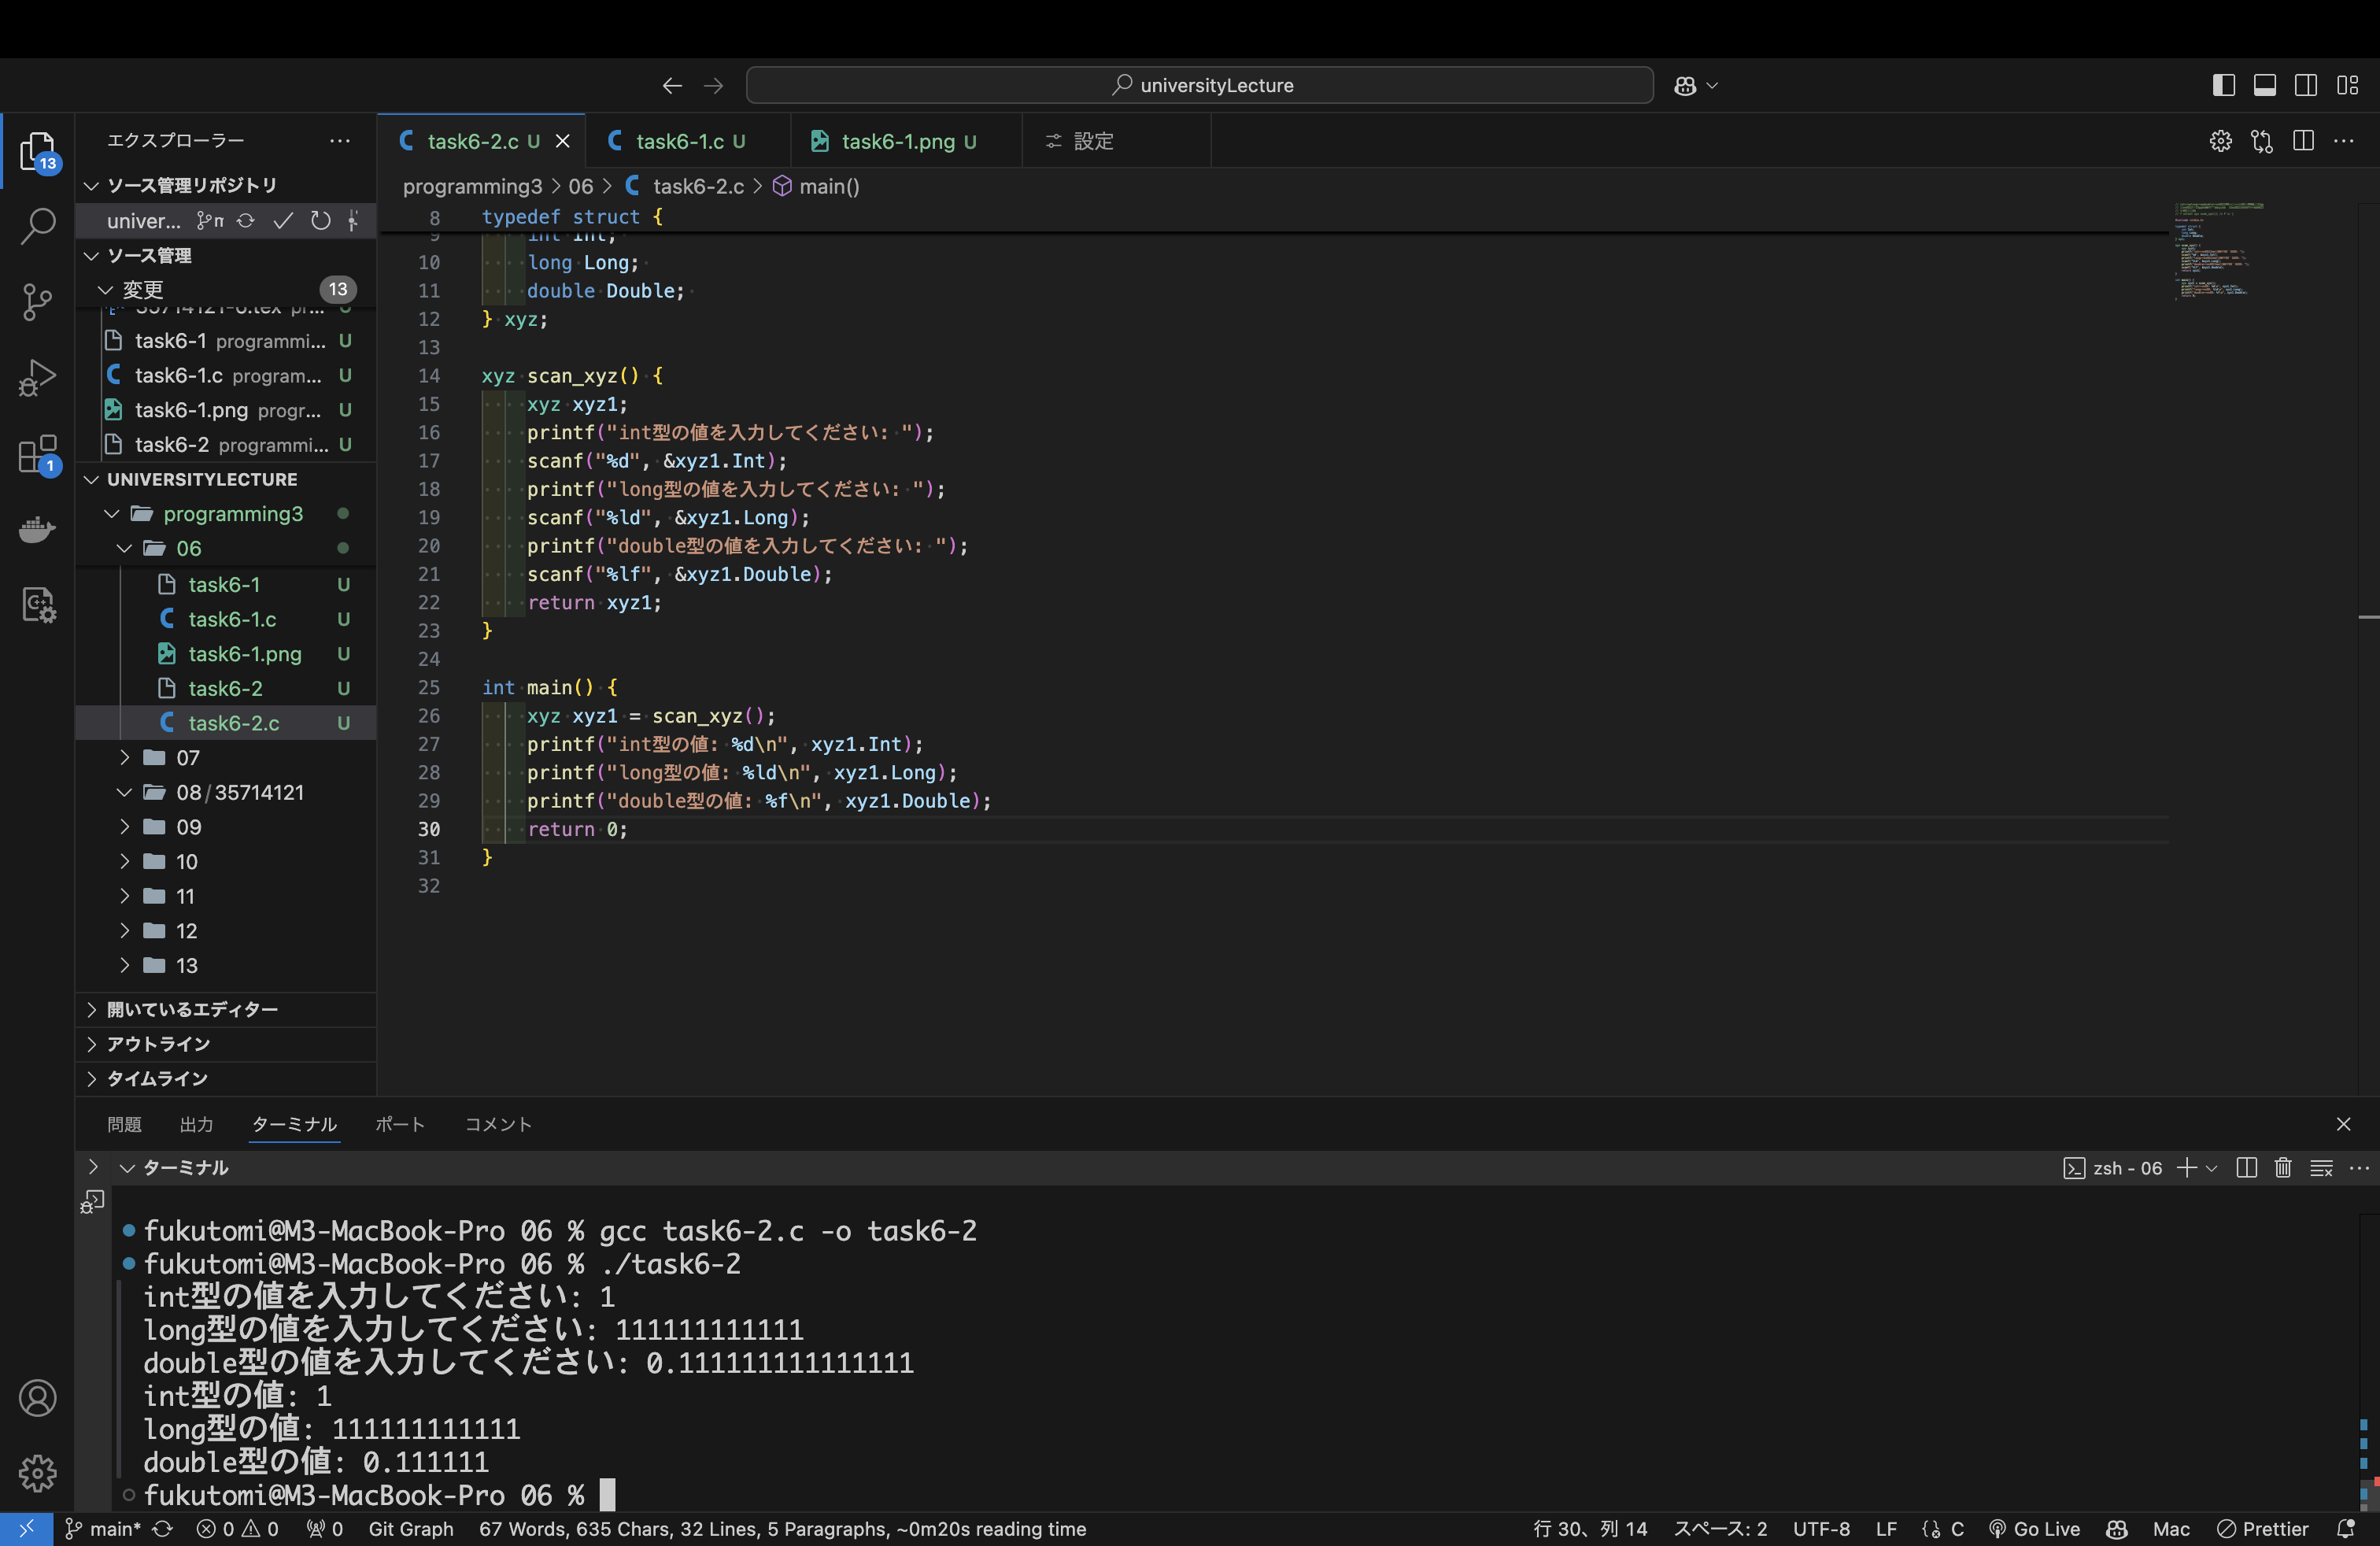
\includegraphics[width=10cm]{task6-2.eps}
  \caption{(ターミナルの部分に実行結果があります)}
  \label{fig:sample2} % ラベル名を変更
\end{figure}

\textmd{コードと結果の説明} \\
メンバの定義だけをした構造体xyzと、scanfでキーボード入力を受けてそれをxyzのメンバに代入し、代入した構造体を返すscan\_xyz関数を作成した。\\
main関数では、scan\_xyz関数を呼び出してxyz型の変数xyz1に代入し、そのメンバを表示した。\\

\end{document}
